\documentclass[12pt]{article}

\usepackage[utf8]{inputenc}
\usepackage{graphicx}
\usepackage{geometry}
\usepackage{titlesec}
\usepackage{xcolor}
\usepackage{listings}
\usepackage{changepage}
\usepackage{hyperref}

\usepackage{multicol}
\setlength{\columnsep}{1cm}
\linespread{1.0}
\renewcommand{\contentsname}{Índice}
\usepackage{mathptmx}

\usepackage{amsmath}
\usepackage{geometry}
\geometry{verbose,a4paper, tmargin=4cm,bmargin=3.5cm,lmargin=2.5cm,rmargin=2.5cm,headsep=2cm,footskip=1.5cm,top=3cm}
\usepackage{fancyhdr}

\begin{document}

\begin{titlepage}
    \centering

    \begin{figure}[ht!]
        \centering
      
\includegraphics[keepaspectratio, width=0.6\textwidth]{logoUSM.png}
    \end{figure}
    \vspace{1cm}
    {\scshape\Large Informe 3, Arquitectura y Organización de Computadores. \par}
    \vspace{1cm}
    {\scshape\Huge Implementación de Flip-Flops D de dos capas para realizar operaciones sobre entradas de 8 bits\par}
    \vspace{1.5cm}
    %{\itshape\Large Sobre sistemas numéricos,  y representación de datos.\par}
    %\vfill
    {\Large Gabriela Acuña, rol 201973504-7.\par}
    \vspace{0.2cm}
    {\Large Profesor Mauricio Solar.}
    \vfill
    {\Large  25 de Junio, 2021 \par}

\end{titlepage}

\tableofcontents
\clearpage


\section{Resumen}
%donde describa brevemente el desarrollo y resultados de la tarea.
Para realizar esta tarea se implementaron 8 flip-flops D de 2 capas, uno para cada bit del numero $X$ de entrada. Cada uno de estos flip-flops se genero desde la configuración conocida de compuertas lógicas. Luego de solucionar esto, se desarrollo individualmente cada uno de los casos posibles según el valor de $M$. Para la suma se utilizo el Full Adder conocido por la tarea anterior, y para la resta se utilizo la implementación propuesta en el enunciado. Para los otros dos casos se utilizaron compuertas de 8 bits. 
 Se consideró una implementación exitosa ya que los resultados obtenidos son iguales a los dados como ejemplo en el enunciado de la tarea. 

\vspace{0.5cm}

%\begin{multicols}{2}
\section{Introducción}
%dejando claro el objetivo de la tarea y cualquier fórmula que utilice

El objetivo de esta tarea fue realizar una implementacio de circuito con memoria interna, compuesta por flip-flops D, para así usar el valor anterior y actual de la variable de entrada $X$ y realizar ciertas operaciones con estos, segun el valor entregado en $M$.

Para el desarrollo de esta tarea se utilizaron Flip-Flops D \footnote{P114 libro} estos se pueden ver en la \textit{figura \ref{fig:ffd2c}} como \textit{FF1} y \textit{FF2}. La union de estos dos FLip-Flops D genera un Flip-Flop D de 2 niveles. Un beneficio de utilizar 2 niveles es que el circuito recuerda su entrada previa y actual en todo momento, sin depender del cambio de ciclo de reloj. Para expander este circuito y utilizarlo en 8 bits, se separo cada uno de los 8 bits de entrada, para recordarlos individualmente, al actual y al anterior. Para no reescribir el circuito muchas veces se utilizo el circuito presentado en la \textit{figura \ref{fig:ffd2c}} como subcircuito, el cual fue nombrado \textit{logicFlipFlop}.

Por otro lado, al igual que para el desarrollo de la tarea pasada, se implemento la suma sin carry de salida a través de un full adder por bit de salida. Para la resta, se utilizo la implementacion de la suma para realizar el atajo presentado en el enunciado que se ve en la \textit{ecuación \ref{eq:resta}}.

\begin{equation}\label{eq:resta}
A - B = A + \overline{B} + 1
\end{equation}

Por ultimo, para realizar el $AND$ y $OR$, se utilizaron compuertas de 2 entradas y 8 bits. Ya que los pines de entrada eran de 8 bits, facilitó bastante el proceso.

\section{Desarrollo}
%donde describa brevemente el desarrollo y resultados de la tarea.
La tarea se organizó a través de subcircuitos, como se puede ver en la \textit{figura \ref{fig:main}} del circuito general de la implementación completa. Por esta razon se procedera a explicar detalladamente el funcionamiento de cada uno de ellos.
\subsection{Circuito de Suma}

Titulado \textbf{Suma} y perteneciente a \textbf{SLogic}, como ya fue mencionado, la base de esta implementación es el circuito conocido \textit{full adder}, que se utiliza para los 8 bits a sumar.

\subsection{Circuito de Resta}

Para el desarrollo de este circuito se utilizo el subcircuito ya explicado de Suma, y con el atajo entregado en el enunciado quedo como una operacion bastante simple, con la negación de $P(X)$ y la suma de la constante 1.

\section{Resultados}



\section{Análisis}
%Los resultados encontrados son los esperados para todas las bases y códigos, considerando que cuando un código se encontraba en la posición de b, se tomaba n como un numero codificado en el mismo.



%\end{multicols}

\section{Conclusión}

%comentando el nivel de finalización de la tarea. Además explique generalmente la función de las distintas bases numéricas y códigos de corrección estudiados en clases.

\newpage

\section{Anexo}

\begin{figure}[h]
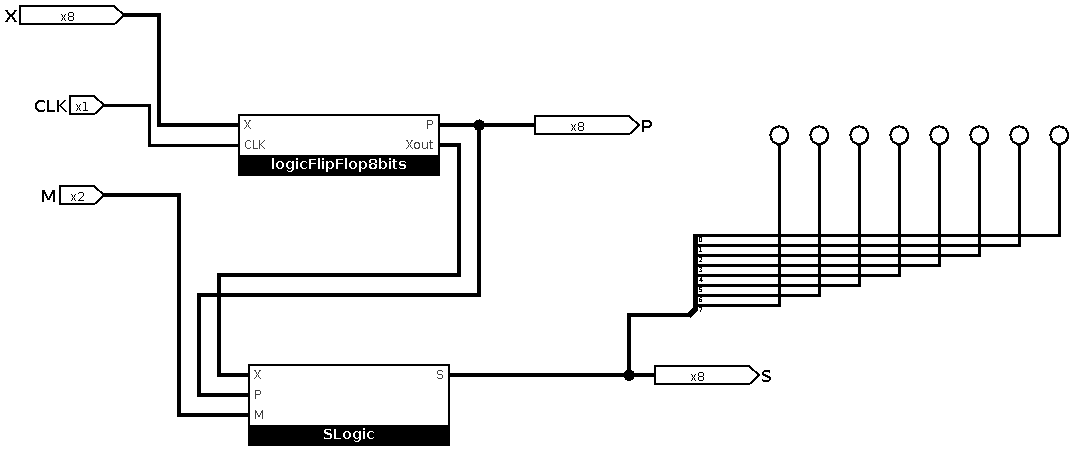
\includegraphics[scale=.4]{main.png}
\caption{Circuito general, con salida en leds y salidas en binario para referencia}
\label{fig:main}
\end{figure}

\begin{figure}[h]
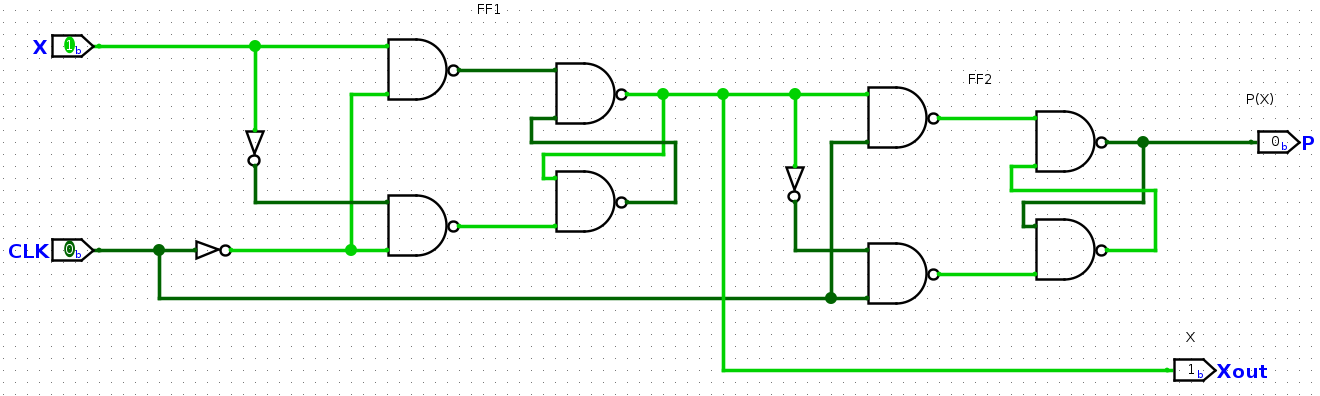
\includegraphics[scale=.3]{logicFlip-FlopD.png}
\caption{Flip-Flop D de 2 capas para 1 bit.}
\label{fig:ffd2c}
\end{figure}

\end{document}